\subsection{Datenfreigabe}
Um Daten vom Privacy Provider nutzen zu können, ist zunächst eine Authentifizierung des Nutzers erforderlich. Hierzu werden die Anmeldedaten in der mobilen App eingegeben. Wird auf den Login-Button geklickt, wird der Nutzer durch den Privacy Provider authentifiziert. Bei diesem Vorgang werden dem Nutzer Lese-, Schreib-, und Ausführungsrechte gewährt, sodass Daten verändert und verschiedene Funktionen ausgeführt werden können. Außerdem wird ein zeitlich begrenzter Schlüssel erzeugt, mit dem der Nutzer Anwendungen Zugriff auf seine Daten gewähren kann. Welche Daten von einer Anwendung lesbar sind, kann der Nutzer in der mobilen App freigeben. Abbildung \ref{fig:accesstoken} zeigt beispielhaft eine Authentifizierung und anschließende Aktualisierung des Standortes des Nutzers mittels des Schlüssels.  

\begin{figure}[!ht]
	\centering
	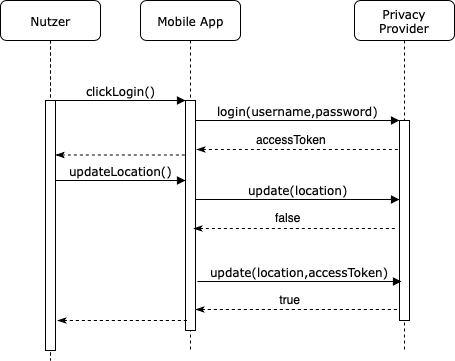
\includegraphics[width=1\linewidth]{Picture/AccessToken.png}
	\caption[Datenfreigabe im Privacy Provider]{Datenfreigabe im Privacy Provider}
	\label{fig:accesstoken}
\end{figure}
